% This is samplepaper.tex, a sample chapter demonstrating the
% LLNCS macro package for Springer Computer Science proceedings;
% Version 2.21 of 2022/01/12
%
\documentclass[runningheads]{llncs}
%
\usepackage[T1]{fontenc}
% T1 fonts will be used to generate the final print and online PDFs,
% so please use T1 fonts in your manuscript whenever possible.
% Other font encondings may result in incorrect characters.
%
\usepackage{graphicx}
% Used for displaying a sample figure. If possible, figure files should
% be included in EPS format.
%
% If you use the hyperref package, please uncomment the following two lines
% to display URLs in blue roman font according to Springer's eBook style:
%\usepackage{color}
%\renewcommand\UrlFont{\color{blue}\rmfamily}
%
\usepackage{tikz, wrapfig}
\usetikzlibrary{positioning}

\begin{document}
%
\title{Active automata learning of an IPsec IKEv1 Server using \textsc{AALpy}}
%
%\titlerunning{Abbreviated paper title}
% If the paper title is too long for the running head, you can set
% an abbreviated paper title here
%
\author{Benjamin Wunderling}

%
\authorrunning{Benjamin Wunderling}
% First names are abbreviated in the running head.
% If there are more than two authors, 'et al.' is used.
%
\institute{Institute of Software Technology, Graz Unversity of Technology, Graz, Austria \\
\email{benjamin.wunderling@gmail.com} \\
Supervised by Bernhard K.~Aichernig}
%
\maketitle              % typeset the header of the contribution
%
\begin{abstract}
Virtual Private Network (VPN) protocols are widely used to create a secure mode of communication between several parties over an insecure channel. A common use case for VPNs is to secure access to company networks. Therefore, errors in VPN software are often severe. IPsec is a VPN protocol that uses the Internet Key Exchange protocol (IKE). IKE has two versions, namely IKEv1 and the newer IKEv2. While IPsec-IKEv2 has been investigated in the context of automata learning, no such work has been performed for IPsec-IKEv1. This paper describes the IPsec-IKEv1 protocol and shows the steps taken to learn the state machine of an IPsec server. We present a learned model and discuss its potential applications for model-based fuzzing and fingerprinting of IPsec implementations.

\keywords{IPsec  \and Automata learning \and \textsc{AALpy} \and VPN.}
\end{abstract}
%
%
%
\section{Introduction}
% background
Virtual Private Networks (VPNs) are used to allow secure communication over an insecure channel. The importance of VPN software has increased dramatically since the beginning of the COVID-19 pandemic due to the influx of people working from home \cite{abhijith2020impact}. This makes finding vulnerabilities in VPN software more critical than ever. IPsec is a VPN protocol and most commonly uses the Internet Key Exchange protocol (IKE) to share authenticated keying material between involved parties. Therefore, IKE and IPsec are sometimes used interchangeably. We will stick to the official nomenclature of using IPsec for the full protocol and IKE for the key exchange only. IKE has two versions, IKEv1 and IKEv2, with IKEv2 being the newer and recommended version \cite{nist791491}. However, despite IKEv2 supposedly replacing its predecessor, IKEv1 is still in widespread use today. This is reflected by the company AVM to this day only offering IKEv1 support for their popular FRITZ!Box routers \cite{avm2022}.
%Problem
State models of protocol implementations are useful tools in testing. They can, e.g., be used to detect software implementations \cite{pferscher2021fingerprinting}, or generate test cases automatically \cite{pferscher2022fuzzing}. One method of generating such models is to use active automata learning. A notable example of an active automata learning algorithm is the $L^*$ algorithm by Angluin \cite{angluin1987learning}. In $L^*$, a learner queries the System under Learning (SUL) and constructs an automaton describing the behavior of the SUL through its responses. This automaton is then compared with the SUL, adapting it if they show different behaviors. Guo et al.~\cite{guo2019model} investigated IPsec-IKEv2 using automata learning \cite{guo2019model}, however so far, no studies have focused on IKEv1 in the context of automata learning. 
% My solution
We learn the state model of a sample IPsec-IKEv1 server using the active automata learning framework \textsc{AALpy} \cite{muvskardin2022AALpy}. We configure \textsc{AALpy} to use $L^*$ automata learning, and construct a custom Python mapper class to facilitate communication between \textsc{AALpy} and the IPsec server.
% Structure of Thesis
In this paper, we first introduce preliminary information on VPNs and automata learning in Section \ref{chap:2}. Section \ref{chap:3} discusses other related work. In Section \ref{chap:4}, we briefly introduce \textsc{AALpy} and our learning setup. Subsequently, we will present our custom mapper class, discussing design choices and implementation difficulties. Finally, we present the learned model and discuss its potential applications and future work in Sections \ref{chap:5} and \ref{chap:6}.


\section{Preliminaries} \label{chap:2} % 1 page
\subsection{Mealy Machines}
Mealy machines are finite state machines where each output transition is defined by the current state and an input. More formally, a Mealy machine is defined as a 6-tuple $M = \{S, S_0, \Sigma, \Lambda, T, G\}$, where $S$ is a finite set of states, $S_0 \in S$ is the initial state, $\Sigma$ is a finite set called input alphabet, $\Lambda$ is a finite set called output alphabet, $T$ is the transition function $G: S \times \Sigma \rightarrow \Lambda$ which maps a state and an element of the input alphabet to another state in $S$ and $G$ is the output function $T: S \times \Sigma \rightarrow S$ which maps a state-input alphabet pair to an element of the output alphabet $\Lambda$.

\subsection{Automata learning}Then
% More on automata learning, in particular L*
Automata learning refers to methods of learning the state model, or automaton, of a system through an algorithm or process. We differentiate between active and passive automata learning. In passive automata learning (PAL), models are learned based on a given data set describing the behavior of the SUL, e.g. log files. In contrast, in active automata learning (AAL) the SUL is queried directly. In this paper, we will focus on AAL and will, moving on, refer to it as automata learning or AAL interchangeably. 

AAL began in 1987 with a paper by Dana Angluin, titled ``Learning regular sets from queries and counterexamples''~\cite{ANGLUIN198787}. In this seminal paper, Angluin introduced the $L^*$ algorithm which is still used for learning deterministic automata. $L^*$ works using a Minimally Adequate Teacher (MAT) model in which a learner queries a teacher about a SUL. The teacher must be able to answer equivalence and membership queries posed by the learner regarding the SUL. Equivalence queries are used to check if a learned model accurately matches the SUL. Membership queries are used to check whether a word is included/accepted. The learner, using the responses to its queries, then updates its model of the SUL. Learned models are commonly represented as Mealy machines, finite-state machines with outputs depending on the current state as well as inputs. The original L* paper learns deterministic finite automata, however the algorithm can be extended to apply to other modeling formalisms including Mealy machines \cite{ShahbazG09}.% in actual paper, a full definition will be given of both $L^*$ and Mealy machines.

\subsection{IPsec}
% More on VPNs, in particular about IPsec
IPsec or IP Security, is a VPN layer 3 protocol used to securely communicate over an insecure channel. It is based on three sub-protocols, IKE, the Authentication Header (AH) and the Encapsulating Security Payload (ESP) protocol. IKE is mainly used to handle authentication and to securely exchange as well as manage keys. Following a successful IKE round, either AH or ESP is used to send packets securely between parties. The main difference between AH and ESP is that AH only ensures the integrity and authenticity of messages while ESP also ensures their confidentiality through encryption.
Compared to other protocols, IPsec offers a high degree of customizability, allowing it to be fitted for many use cases. However, in a cryptographic evaluation of the protocol, Ferguson and Schneier \cite{ferguson1999cryptographic} criticize the complexity arising from the high degree of customizability as the biggest weakness of IPsec. To address its main criticism, IPsec-IKEv2 was introduced in RFC 7296 to replace IKEv1 \cite{kaufman2014internet}. Nevertheless, IPsec-IKEv1 is still in wide-spread use to this day, with the largest router producer in Germany, AVM, still only supporting IKEv1 in their routers \cite{avm2022}. We use IPsec-IKEv1 with ESP in this paper and focus on the IKE protocol as it is the most interesting from an AAL and security standpoint. % this part could maybe be moved to the introduction, not sure

\begin{wrapfigure}{1}{0pt}
	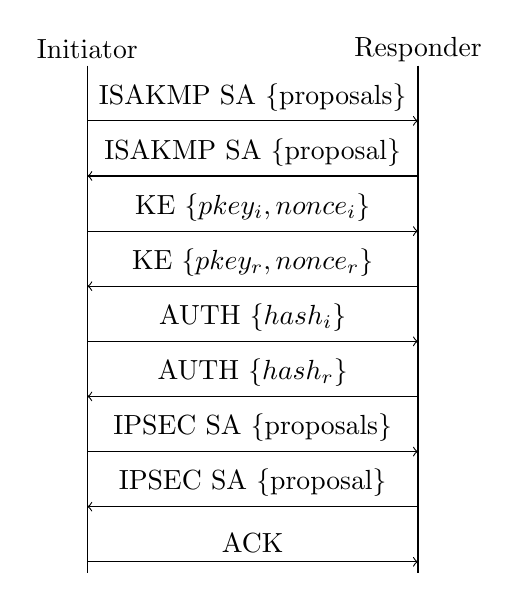
\begin{tikzpicture}[scale=0.7]
	\draw (-3,0) -- (-3,-9.2) (3,0) -- (3,-9.2);
	\node at (-3,.3) {Initiator};
	\node at (3,.3) {Responder};
	\draw[->] (-3,-1) -- node[midway,above] {ISAKMP SA \{proposals\}} (3,-1);
	\draw[<-] (-3,-2) -- node[midway,above] {ISAKMP SA \{proposal\}} (3,-2);
	\draw[->] (-3,-3) -- node[midway,above] {KE $\{pkey_i, nonce_i\}$} (3,-3);
	\draw[<-] (-3,-4) -- node[midway,above] {KE $\{pkey_r, nonce_r\}$} (3,-4);
	\draw[->] (-3,-5) -- node[midway,above] {AUTH $\{hash_i\}$} (3,-5);
	\draw[<-] (-3,-6) -- node[midway,above] {AUTH $\{hash_r\}$} (3,-6);
	\draw[->] (-3,-7) -- node[midway,above] {IPSEC SA \{proposals\}} (3,-7);
	\draw[<-] (-3,-8) -- node[midway,above] {IPSEC SA \{proposal\}} (3,-8);
	\draw[->] (-3,-9) -- node[midway,above] {ACK} (3,-9);
	\end{tikzpicture}
	\caption{IKEv1 between two parties}
	\label{fig:IKEv1}
\end{wrapfigure}

The IKEv1 protocol works in two main phases, both relying on the Internet Security Association and Key Management Protocol (ISAKMP). A typical exchange between two parties, an initiator and a responder, can be seen in Figure \ref{fig:IKEv1}. In phase one (Main Mode), the initiator sends a Security Association (SA) to the responder. A SA essentially details important security attributes for a connection such as the encryption algorithm and key-size to use, as well as the authentication method and the used hashing algorithm. These options are bundled in containers called proposals, with each proposal describing a possible security configuration. While the initiator can send multiple proposals to give the responder more options to choose from. In comparison, the responder must answer with only one proposal, provided it supports one of the suggestions. Subsequently, the two parties perform a Diffie-Hellman key exchange and exchange nonces to generate a shared secret key. This secret key is used as a seed key for all further session keys. Following a successful key exchange, all further messages are encrypted. Finally, both parties exchange hashed authentication material (usually pre-shared keys or certificates) and verify the received hash. If successful, a secure channel is created and used for phase two communication.
The shorter phase two (Quick Mode) begins with another SA exchange. This time, however, the SA describes the security parameters of the ensuing ESP/AH communication. This is followed by a single acknowledge message from the initiator to confirm the agreed upon proposal. After the acknowledgment, all further communication is done via ESP/AH packets. 


\section{Related Work} \label{chap:3} % 1/2 page
% Discuss related papers (chinese, other similar protocols?)
Model learning of other network protocols like SSH \cite{fiteruau2017model}, or TCP \cite{fiteruau2016combining} has been performed in the past, with learned models being used for model checking the learned protocols. Both Novickis et al. \cite{novickis2016protocol} and Daniel et al. \cite{daniel2018inferring} learned models of the related OpenVPN protocol \cite{novickis2016protocol} and used the learned models for fuzzing. In a work by Pferscher and Aichernig \cite{pferscher2021fingerprinting}, learned models were used to fingerprint Bluetooth Low Energy devices (BLE). Guo et al. \cite{guo2019model} used automata learning to learn and test the IPsec-IKEv2 protocol. In contrast with our work, they used the LearnLib library for automata learning and utilized the learned model for model checking.

\section{Learning IPsec} \label{chap:4} %or other title --> method, eihter way, decribe design decisions here ~1.5 pages
\subsection{Environment Setup} % 1/2 page
% describe VMs, IPsec server software, configuration etc
We developed and tested our mapper class using two VirtualBox 6.1 Virtual Machines (VMs) running standard Ubuntu 22.04 LTS distributions. All communication took place in an isolated virtual network to eliminate possible external influences. During learning, all power saving options and similar potential causes of disruptions were disabled. The IPSec server was restarted before each learning attempt. We designated one VM as the initiator and one as the responder to create a typical client-server setup. The open source IPsec implementation Strongswan\footnote{https://www.strongswan.org/} was installed on the responder VM and set to listen for incoming connections from the initiator VM. We used the Strongswan version US.9.5/K5.15.0-25-generic, installed using the default Ubuntu package manager, apt. The Strongswan server was configured to use pre-shared keys for authentication and default recommended security settings. Additionally, it was configured to allow unencrypted notification messages, which we used in our interface to reset the connection. The provided Python script, \emph{IPSEC\_IKEv1\_SUL} demonstrates how we use the learning library \textsc{AALpy} in conjunction with our custom mapper to communicate with and learn the model of an IPSec server.

\subsection{Learning Setup} % half - quarter page
\textsc{AALpy} is an automata learning library written in Python. It boasts support for deterministic, non-deterministic and stochastic automata, with support for various formalisms for each automata type. We used deterministic Mealy machines to describe the IPsec server. However, learning automata with \textsc{AALpy} follows the same pattern, regardless of the type of automata.

\begin{figure}
	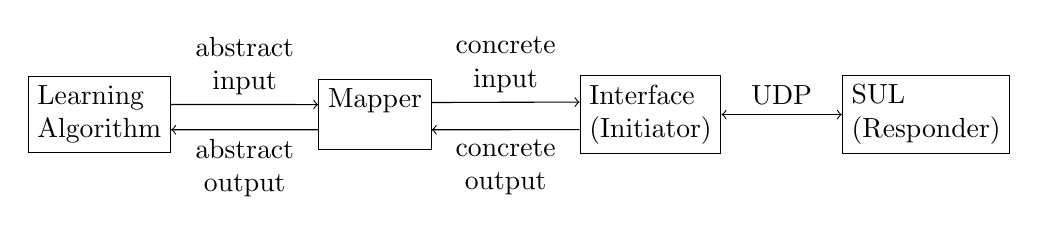
\begin{tikzpicture} 
	\node (n1) [draw, minimum width=4em, align=left] at (0,1) {Learning\\Algorithm};
	\node (n2) [draw, minimum width=4em, align=left] at (3.5,1) {Mapper\\};
	\node(n3) [draw, minimum width=4em, align=left] at (7,1) {Interface\\(Initiator)};
	\node(n4) [draw, minimum width=4em, align=left] at (10.5,1) {SUL\\(Responder)};
	\draw [->] (n1.8) -> (n2.170) node[midway,above,align=center] {abstract\\input};
	\draw [->] (n2.195) -> (n1.348) node[midway,below,align=center] {abstract\\output};
	
	\draw [->] (n2.12.9) -> (n3.170) node[midway,above,align=center] {concrete\\input};
	\draw [->] (n3.192.5) -> (n2.345) node[midway,below,align=center] {concrete\\output};
	
	\draw [<->] (n3) -> (n4) node[midway,above,align=center] {UDP};


	\end{tikzpicture} 
	\caption{Automata Learning Setup}
	\label{fig:AALSetup}
\end{figure}
Figure \ref{fig:AALSetup} gives an overview of the learning process, adapted from Tappler et al.~\cite{tappler2017}. To begin, the learning algorithm sends abstract inputs chosen from the input alphabet to the mapper class, which converts it to concrete inputs. The abstract inputs are then sent to the SUL, by means of a communication interface. In our case, the mapper class comprises the major portion of our work and converts the abstract words into actual IPsec packets that can be sent to the SUL Strongswan server via UDP packets. This separation between abstract and concrete in/outputs allows for easy future modifications to the message implementations, including fuzzing support, as well as increasing the readability of our code.

To begin learning an automaton with \textsc{AALpy}, we must first choose a suitable input alphabet encompassing the language known by the server, as well as the learning algorithm to be used. Our chosen input alphabet consists of the initiator-to-responder messages shown in Figure \ref{fig:IKEv1}. We use the $L^*$ algorithm for learning with an equivalence oracle that provides state-coverage by means of random walks. The chosen equivalence oracle is used by the learning algorithm to test for conformance between the current hypothesis and the SUL, giving either a counterexample on failure, or confirmation that we have learned the SUL. Additionally we defined a \emph{step} and \emph{reset} method. We use \emph{step} to execute one input action from the current query and \emph{reset} to revert the SUL to an initial clean state. We also enabled several optional \textsc{AALpy} features including caching and non-determinism checks to improve the learning process. \\

Our mapper class implements methods for each communication step in a typical IPsec-IKEv1 exchange, as described in Section \ref{chap:2}. We use the Python library Scapy\footnote{https://scapy.readthedocs.io/en/latest} to construct ISAKMP packets as required by the IKEv1 protocol. This approach allows us to change fields and values of generated packets at will, opening the possibility of fuzzing for our future work. Parsing was made more difficult by the fact that Scapy does not support all the packets required by IPsec-IKEv1. To solve this problem, we implemented the missing packets in the Scapy ISAKMP class and used this modified version. 

The IPsec packets generated by the mapper class are then passed on to our communication class, which acts as an interface for the SUL and handles all incoming and outgoing UDP packets. Additionally, it parses responses from the SUL into valid Scapy packets and passes them on to the mapper class. The mapper class then parses the responses received from the communication interface and returns an abstract output code representing the received data to the learning algorithm. \\

As messages will be sent in random order during learning, we require a robust framework that correctly handles en/decryption of messages. For key management, we simply store the current base-keys but keep track of Initialization Vectors (IVs) on a per-message id (M-ID) basis. Additionally, we keep track of the M-IDs of server responses to detect and handle retransmissions of old messages. Each request, we store the response for use in the next message and update affected key material as needed. Most notably, the IVs are updated almost every request and differ between M-IDs. Informational requests also handle their IVs separately. For each request that we send, if available, we try to parse the response, decrypting it if necessary and resetting or adjusting internal variables as required to match the server. This is required to continuously be able to parse server responses and extract meaningful information.

Automata learning requires a SUL reset method to be able to return to an initial starting point after each query. We implement this using a combination of the ISAKMP delete request and general ISAKMP informational error messages. While delete works for established connections in phase two of IKE, we require informational error messages to trigger a reset in phase one, as delete does not work here sufficiently. Implementation was hindered at times by unclear RFC-specifications, but this was overcome by manually comparing packet dumps and Strongswan logs to fix encryption errors.\\

Since the server occasionally exhibits non-deterministic behavior, we had to implement methods of counteracting it. The first solution is to catch these non-determinism errors as they occur and simply repeat the offending query several times. If upon the first rerun the non-determinism does not occur again, we accept the existing value as the correct one and continue. If however, it persists for a set amount of repetitions with the same constant server response, we assume that the original saved response was incorrect and update it to the new one. With this non-determinism correcting added, the automata learning works with no errors and the learned automata are consistent with one another. Additionally, making use of timed waits after each communication to give the server time to respond also helps decrease the number of non-determinism errors that have to be caught. The resulting models still had occasional differences, but on average looked like the one shown in Figure \ref{fig:learnedmodelret}.

Another, more reliable fix, but with some downsides, involves server retransmission messages. Examination of outliers among the learned automata led to the discovery that close to all non-comforming automata were caused by these so-called retransmissions. Essentially, the IKE specification allows for previous messages to be retransmitted if deemed useful. A possible trigger could be the final message of an IKE exchange being skipped / lost. For example, if instead of an \emph{AUTH} message, the server receives a phase two \emph{IPSEC SA} message, the server would not know if it missed a message or if their was an error on the other parties side. In this case, the Strongswan server reacts by retransmitting the previous message, prior to the missing one in an attempt to signal to the other party, that they should resend the missing message. 
While interesting for fingerprinting, we wanted a deterministic automaton as a base case for automata-based fuzzing, so we implemented checks in our mapper to allow the ignoring of retransmissions. The retransmission-filtering can be easily enabled or disabled through a simple flag and works by checking the message ID of incoming server responses against a list of previous message IDs (excluding zero, as it is the default message ID for phase one). If a repeated message ID is found, it is flagged as a retransmission and depending on the current filtering rule, ignored. With this addition, the IPSec server became 100\% deterministic, allowing the learning of very clean automata, as shown in Figure \ref{fig:learnedmodel}. The downside of this method is, that it completely ignores the retransmissions, which could be a good source of information for fingerprinting purposes.

\section{Evaluation} \label{chap:5} % 1.5 pages
Both models, shown in Figures \ref{fig:learnedmodelret} and \ref{fig:learnedmodel}, were learned from a Linux Strongswan U5.9.5 server, with a typical P2P PSK configuration. The first model, seen in Figure \ref{fig:learnedmodelret} was learned with retransmissions enabled. This model took an average of 300 minutes to learn over 5 learning rounds and consists of 13 states. Of the 300 minutes, roughly 75\% were used for state exploration or output queries and 25\% for conformance checking. 786 output queries were performed in roughly 6600 steps. On average, three to four non-determinism errors were caught and fixed per learned model, however it should be noted that the learned automata for runs that required non-determinism fixing and those that did not are identical. We therefore assume it to be caused by retransmission timing inconsistencies occurring rarely on the server, causing non-deterministic behavior. \\

A strong separation can be observed between states zero through three and four through twelve. This separation matches the separation of IKEv1 into two phases. Once phase one has completed, phase one messages should be ignored by the IPsec server and the learned automata reflects this behavior. Another interesting behavior is exhibited in states S6 and S10, where an input of \texttt{SA\_main}, \texttt{authenticate} or \texttt{key\_ex\_main}, all phase one inputs, which are usually ignored in phase two, returns a valid and unexpected \texttt{IPSEC\_SA} response. This behavior seems to be a specific chain of inputs that causes a retransmit of a previous response, which then does not match the input, which does in fact get ignored by the server. Some of the None responses are due to design choices in the mapper class implementation, as some impossible cases were simplified to save time. For example, if no key-exchange has yet occurred, the client will not be able to send sensible encrypted data, so the mapper class simply returns None. While observing the behavior of the server when exposed to completely non-sensible input is interesting from a fuzzing standpoint, as all specifications state that the encryption requires a prior keying procedure, we decided to ignore those few cases. However, for future work in the field of fuzzing, these edge-cases should be considered as well.\\

Another noticeable property of the learned automata, is that past state S2, no paths lead back to the initial state. This is due to the fact that we did not include the delete command in the alphabet for this learned model. Adding delete adds transitions from every state back to the initial one, but also dramatically increases the runtime.

To investigate interesting behavior seen on the learned model, we developed a small testing framework that allows one to execute individual runs very simply. This allowed us to quickly perform sanity-checks for our model and verify that individual runs match the behavior shown by the model. 


% the model
\begin{figure}[!h]
	\centering
	\includegraphics[width=1\linewidth]{LearnedModelRet}
	\caption[Learned Model]{Strongswan Server Automata with retransmissions}
	\label{fig:learnedmodelret}
\end{figure}

In contrast, the second model, shown in Figure \ref{fig:learnedmodel} was learned while filtering out retransmissions as described in Section \ref{chap:4}. Additionally, several different error messages are grouped together for readability. The model tool a total of just over 30 minutes to learn over 2 learning rounds and consists of 6 states. The split between state exploration and conformance checking is largely the same, but only 197 output queries were required over a total of 961 steps. On average, zero non-determinism errors occurred and had to be filtered.

We can see when comparing the two automata, that the phase one section is identical between both automata. This is likely due to the fact, that most differences were caused by retransmissions which only occur after phase one is completed. In the second model, we can clearly distinguish between the individual phases of the IPsec IKEv1 exchange. The clean automaton makes it easy to see, that after a connection has been established, we can still create new connections / restablish existing ones by sending another \emph{IPSEC SA} message and then acknowledging it.


% the clean model
\begin{figure}[!h]
	\centering
	\includegraphics[width=1\linewidth]{LearnedModel}
	\caption[Learned Model]{Strongswan Server Automata without retransmissions}
	\label{fig:learnedmodel}
\end{figure}

\section{Conclusion and Future Work} \label{chap:6} % half page
The learned models show that our \textsc{AALpy} mapper class works as intended and can be used to learn the behavior of an IPsec server. We discussed the implementation problems that arose and described our solutions to those problems. Particularly noteworthy are our contributions to the Scapy ISAKMP module and our non-determinism handling, as well as our \emph{reset} method. Looking towards potential use cases for our learned automata, our focus on keeping generated packet fields easily modifiable makes automata-based fuzzing a straightforward extension of our work. Future work could also go into improving the performance and error-handling of our mapper class. Additionally, comparing the learned model with those of other servers and other software versions could prove to be an interesting application area. \pagebreak


%
% ---- Bibliography ----
%
% BibTeX users should specify bibliography style 'splncs04'.
% References will then be sorted and formatted in the correct style.
%
\bibliographystyle{splncs04}
\bibliography{bibliography}
\end{document}
